\chapter{Deep Learning Models for Fetal Pain Assessment}

In this chapter, we present some background topics recommended for a better understanding of our work and later explain the methodology that was used to conduct our experiments.

\section{Background}

When dealing with image classification task, traditional machine learning algorithms require hand-engineered features, like filters and descriptors, to be used as an input for algorithms. The algorithms were then trained to find patterns in these features capable of distinguishing between different classes.

Neural networks, on the other hand, have the advantage of being able to learn these features directly from the data, which makes the process of feature engineering a lot simpler and achieves better results in most cases. Furthermore, the recent advances in Deep Neural Networks have taken these capabilities to a new level. They not only win most of the competitions in the field but also achieve state of the art results in a wide range of real applications. One type of network that was responsible for these results is Convolutional Neural Networks (CNNs).

\subsection{Convolutional Neural Networks}

Convolutional Neural Networks are similar to traditional Neural Networks. They both have an input layer which receives the data, followed by hidden layers with numerous neurons with weights and biases capable of learning the characteristics of the data, and an output layer at the end which makes the classification. The main difference is that CNNs assume the input has some spatial relationship, which is a pattern present in images, so knowledge of where pixels are located in reference to each other is preserved. CNNs are then capable of extracting these features and capture patterns that would not have been possible if we used traditional networks. To extract these features, the networks use two primary operations: convolution and pooling.

Convolutions are mathematical operations that act as learnable filters to capture patterns in the images. These filters usually are small in terms of dimension, sometimes 3x3 or 5x5 matrices, also called Kernels. Each one of them convolves across the width and height of the input image and compute dot products that produce an activation map of the image. These activation maps, once learned, will be able to detect features in the images, such as edges, corners, or color shifts. 

Pooling is another mathematical operation responsible for reducing the spatial size of the convolved feature. These series of transformations reduce the dimensionality of the data and makes it possible to process images of high resolution. 

As multiple convolutional and pooling layers are stacked, the network becomes able to detect more complex patterns that are composed of multiple inputs of different feature extractors in the first layers. \citep{} has demonstrated a good visualization of this process. 

\subsection{Transfer Learning}

Transfer Learning is a technique commonly used in machine learning where a learning model that was originally developed for one task is then reused on a second related task. It comes from the assumption that what has been learned in one setting can be used to improve optimization in another setting.

The number of parameters present in a CNN is very high, which requires a large amount of training data to tune the network for making precise predictions. As an example, a dataset that is commonly used in the field, ImageNet, contains 1.2 million images and has 1000 categories to classify. Besides that, computational power to train a network in such a large dataset is also another obstacle.

In this scenario, the solution of using transfer learning trough pre-trained networks arises as a solution. In this process, the weights and biases from a network trained in another task, are reused to train a new similar task.

Even though computing power increased a lot ever since CNNs were invented, they still require a significant amount of hours to be trained. So this is also a computationally wise approach.

Thus, transfer learning is considered in both scenarios. First, when we do not have enough data, second, when we do not have enough computational power to train a network from scratch.

The problem of having little annotated data is common in the medical field, and thus transfer learning is often used.

The idea behind is inspired by human behavior, where sometimes we can use expertise in solving one problem to learn to solve another one.

\subsection{Data Augmentation}

\subsection{Visual Explanations}

\section{Methodology}

\subsection{Image Sampling}

It is common to have a small number of data to work with as this is a very hard data to collect. Only a small percentage of pregnancies require intra-uterus intervention prior to birth, and thus fetal anesthesia is a relatively rare procedure. Because of that, it is common for studies in the filed to also have a small N, like these ones cite{}.

To deal with the limited amount of data, we've decided to bring the data to another dimension, we reduced the space from videos to images. In other to do this, we decided to sample the videos at the hate of every 2 seconds. With these processes, we created a total of 268 images.

But as the images were recorded from ultrasound machines, they depend on the calibration by the doctors to capture the exact section of the 3-dimensional space where the fetus face is. Because of this, it is common for this type of image to have a lot of noise, and thus some of the sampled images did not contain a clear face of the fetus. This was a problem, as we had a significant number of images, and manual selection would not only be hard but also non-deterministic.

To overcome this issue, we decided to use a neural network capable of detecting facial landmarks, like the nose, the mouth, and the eyes. The network we used was the Multi-task Cascaded Convolutional Networks (MTCNN) developed by \cite{ZhangZL016} which was created to identify faces in images. It worked surprisingly well in our domain, even though the images had quite different characteristics.

With this process, we were able to filter out our dataset of images from 268 to 145 and we're sure the images contained a clear face. The network also returned a confidence number of which it found the face in the image, and we've used only confidences of over 95\%, which on manual inspection was very reliable, with just 6 errors that were removed manually.

With the position of the facial landmarks, another process was to crop the images around the face of the fetus. This cropping is done just by adding padding to the places where the image was. This process is achivable after we have the positions of the landmarks returned through the MTCNN. This also makes face alignment possible. This way, we avoid the blurred surroundings around the fetus which contains non-distinguishable parts. 

At this point, manual inspection was needed in other to separate the images back into the three groups. With the resting images, it was easy as all the frames were from resting positions. But with the ones from anesthesia and from the horn we had to split the data between before the stimulus and after it. This was not a though process as we knew exactly when the stimuli were applied and a clear difference in the facial expression could be noted. After this step, we ended up with 117 images which had a clear face on it. An example of cropping can be seen on Figure \ref{fig:cropping}.

\begin{figure}[h!tp]
    \centering
    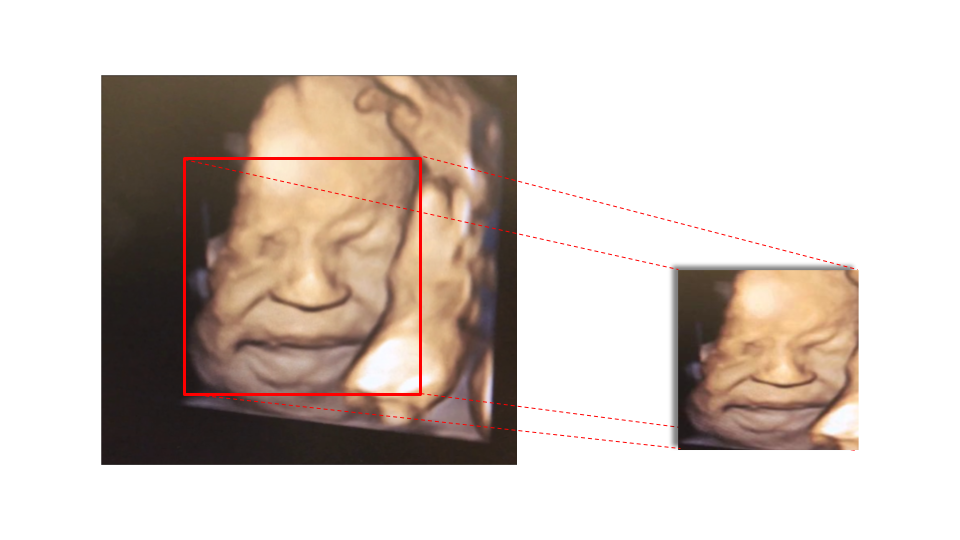
\includegraphics[width=.9\textwidth]{imgs/chap3_cropping.png}
    \caption{Image cropping with MTCNN}
    \label{fig:cropping}
\end{figure}

\subsection{Data Augmentation}

Even though we had increased the size of the dataset by turning the videos into images, it was still considered a small dataset for deep learning models. To further augment our chances of succeeding, we have applied the use of data augmentation techniques to increase the variability of our data. The effectiveness of such a technique has been demonstrated by \cite{abs-1712-04621} and is widely used in the field.

There is a range of possibilities for using data augmentation, the ones we've chosen are:

* Horizontal flip, which consists of mirroring the image horizontally. 
* Rotation, which consists in applying small rotations to the image.
* Zoom, which consists of zooming in the image.
* Lightning, which consists of changing the brightness and the contrast of the image.
* Warping, which consists of adding distortions to the image. 

All of these methods have a probability of being applied and can be used in combination with each other. Thus for each image, given the probability, a combination of these techniques would be applied. Some examples of these different combinantions of data augmentation with the same image are shown on Figure \ref{fig:data_augmentation}.

\begin{figure}[h!tp]
    \centering
    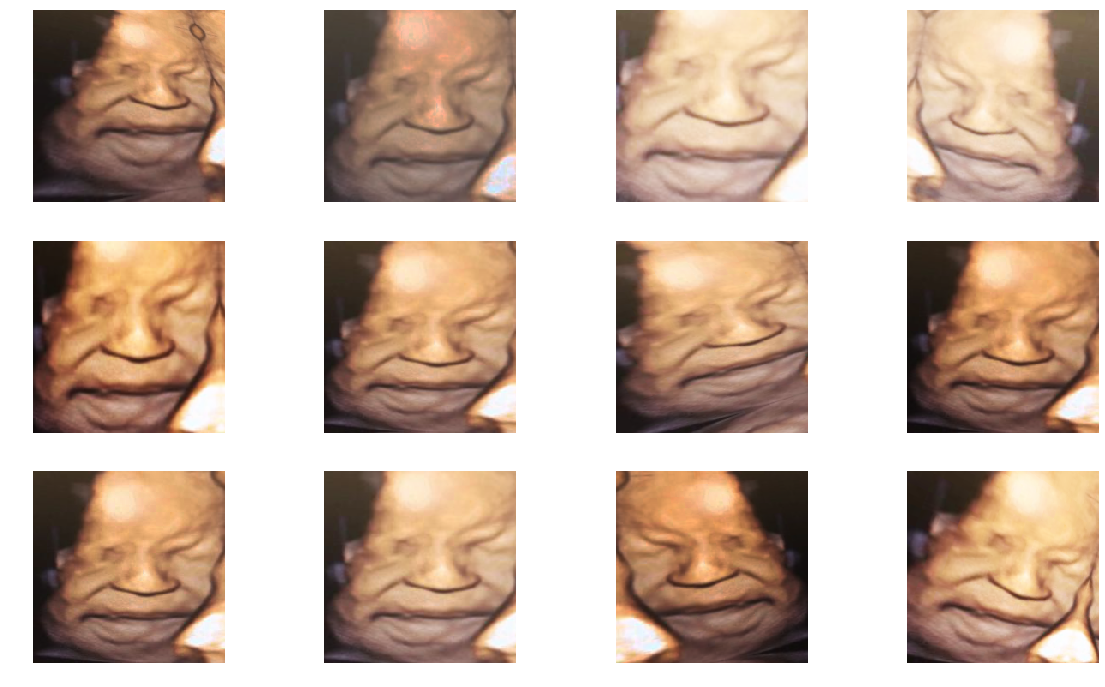
\includegraphics[width=.9\textwidth]{imgs/chap3_data_augmentation.png}
    \caption{The same image with different data augmentation applied}
    \label{fig:data_augmentation}
\end{figure}

To further experiment with this process, we have compared 3 sets of intensity in the changes. A smooth, which does more subtle changes, a medium one, which intensifies a little bit and a more aggressive one, which heavily transforms the images.  
\subsection{Network Architecture and Transfer Learning}

The network used was VGG with a pre-trained model on VGG Face, developed by \cite{ParkhiVZ15}.



